\chapter{Downwash Estimation}

In order to evaluate the characteristics of longitudinal stability of an aircraft it's necessary to assess the flow direction aft of the wing. The contribution of horizontal tail surface to the airplane equilibrium and stability, in fact, depends seriously on the flow direction. The pourpose of this chapter is to introduce and evaluate the downwash gradient due from the wing's vortex system, considering a dipendence of the downwash angle from the absolute angle of attack. 

\section{Theoretical background}

Due to the finite extention of the wing the lift distribution in span is not uniform. For this reason the difference of pressure between upper and lower surfaces generates a movement of air aroud the wingtips. The tendency is for particles of air to move from the region of high pressure around the wing tip to the region of low pressure (for positive lift from the lower wing surface to the upper surface). This made the wing's vortex system that consisting of the bound vortex, located at the wing quarter chord and a vortex sheet which rolling up, at the wing tip, in two trailing vortex.\cite{PerkinsHage} \cite{Jacobs:NACA:Rep:648} \\ 

\begin{figure}[H]
\centering
{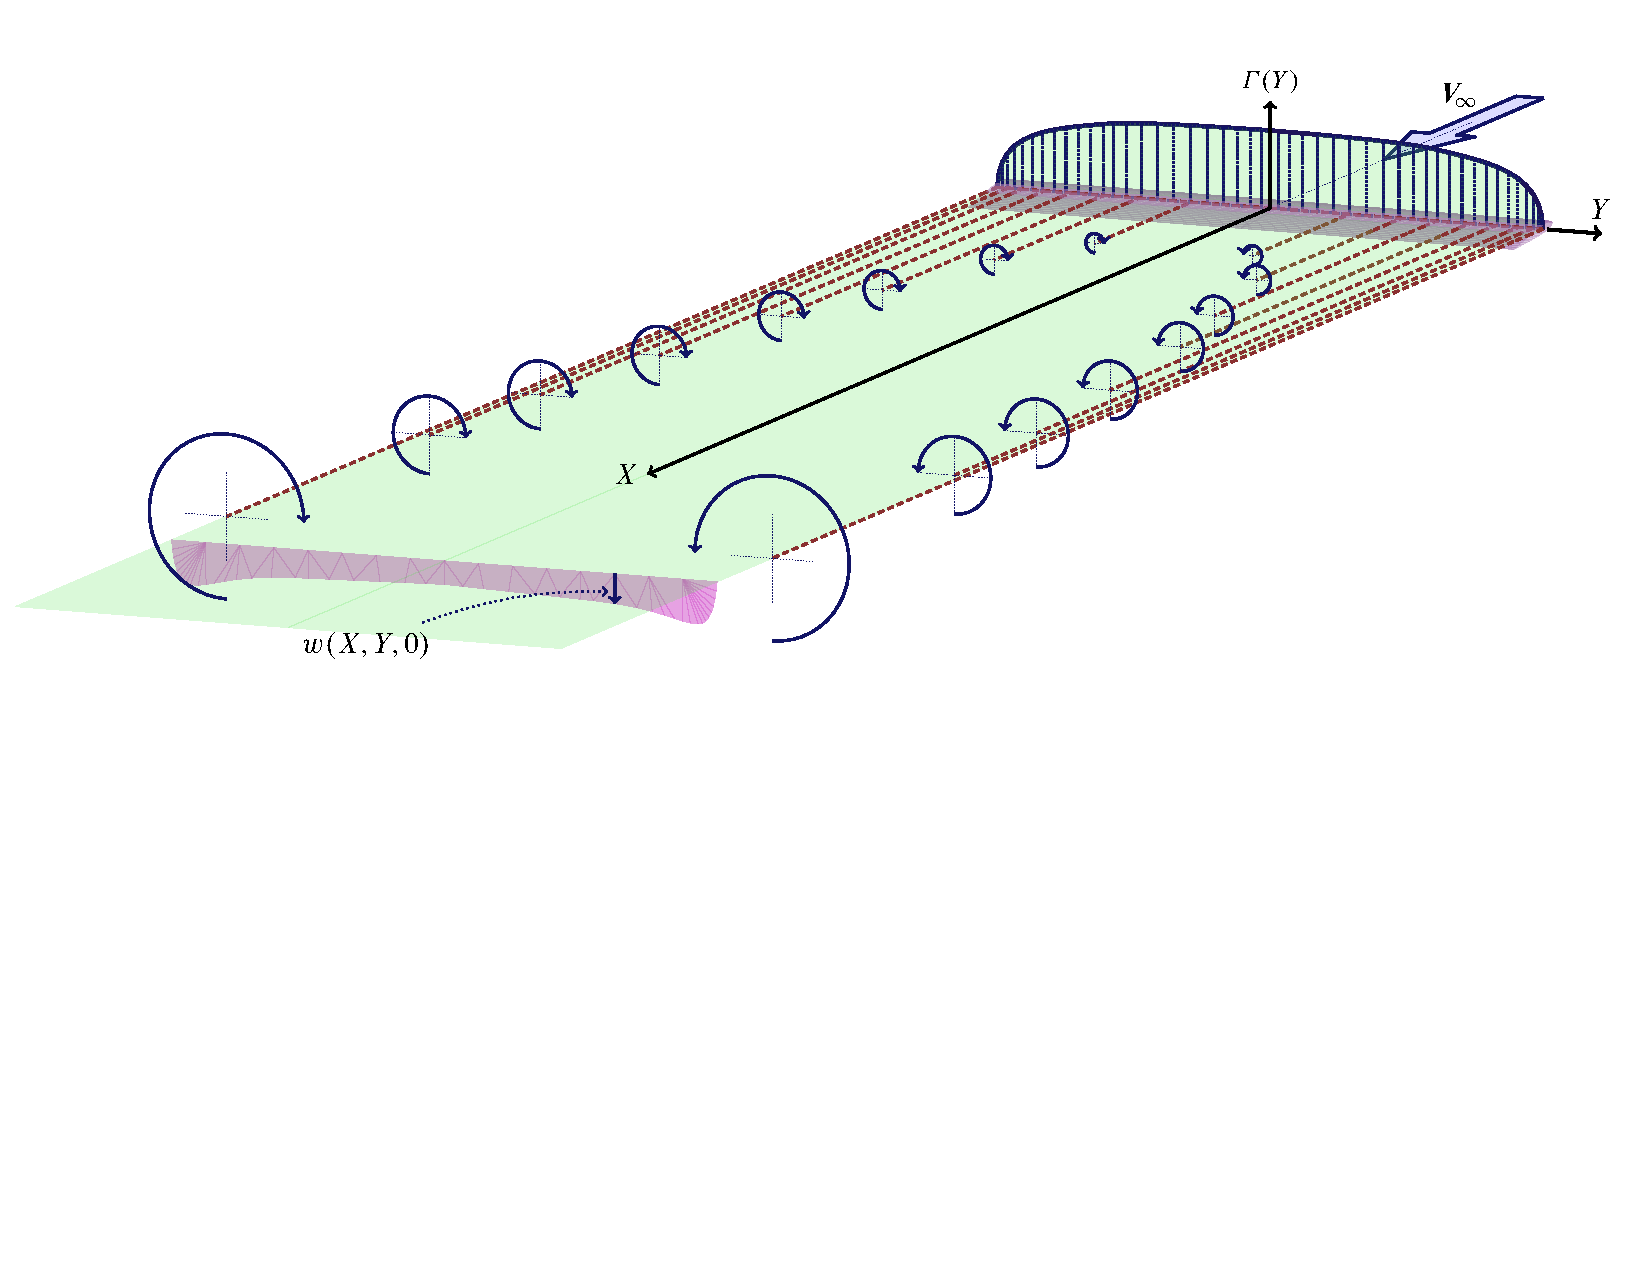
\includegraphics[height=6cm]{Immagini/wing_vortex_sheet3.pdf}} 
\caption{The wing vortex sheet.}
\end{figure}

The main effect of this vortex system is to deflect the airflow behind the wing downward relative to the direction of freestream flow. This angle of deviation is known as {\itshape Downwash Angle} $\epsilon$. This phenomenon occurs for every lifting surface, but in subsonic flow a lifting surface also affects the flow forward of itself. In this region the vortex creates an {itshape Upwash}, that is an upward flow deflection.\\


\begin{figure}[H]
\centering
{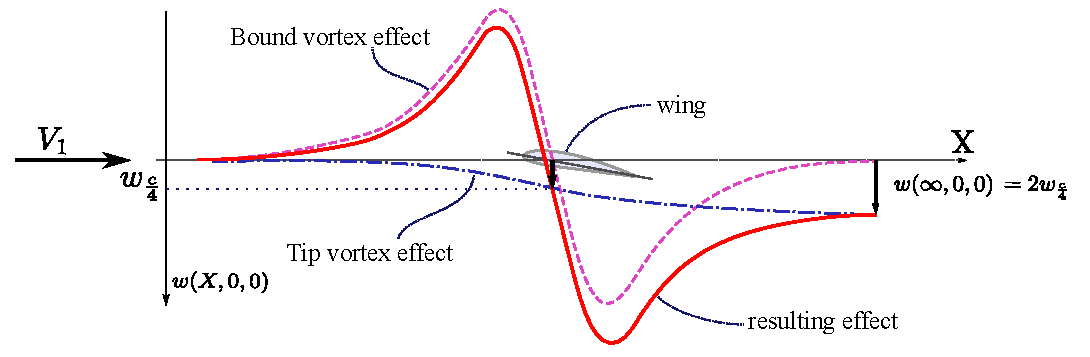
\includegraphics[height=5cm]{Immagini/wing_upwash_downwash.pdf}} 
\caption{Upwash and Downwash in a finite wing.}
\end{figure}

As consequence of the downwash behind the wing, the local angle of attack on the horizontal tail is reduced by  $\epsilon$. In order to evaluate the dlow direction behind the wing, an other important parameter id the change in downwash angle with angle of attack, that is the {\itshape Downwash Gradient } $\frac{d\epsilon}{d\alpha}$.\\
This parameter depends principally on the location of the horizontal tail with respect to the wing and the vortex plane. As first approssimation this value could be considered constant in alpha, but more accurately it's possible to evaluate this dependence considering the reference variable for the calculation of the distances. \\ \\

In order to evaluate the downwash gradient it refers to fig. \ref{PerkinsDownwash}, where ``$r \frac{b}{2}$''  is the distance between the aerodynamic center of wing and the aerodynamic center of the horizontal tail. This is a geometric an fixed distance. Conversely,  in order to have a greates accuracy it's possible to consider the distance ``$m  \frac{b}{2}$'' variable with the angle of attack. Properly this is the distance between the horizontal tail and the vortex shed plane, but it's possible to approximate it with the distance between the horizontal tail and the wing root chord.

\begin{figure}[H]
\centering
{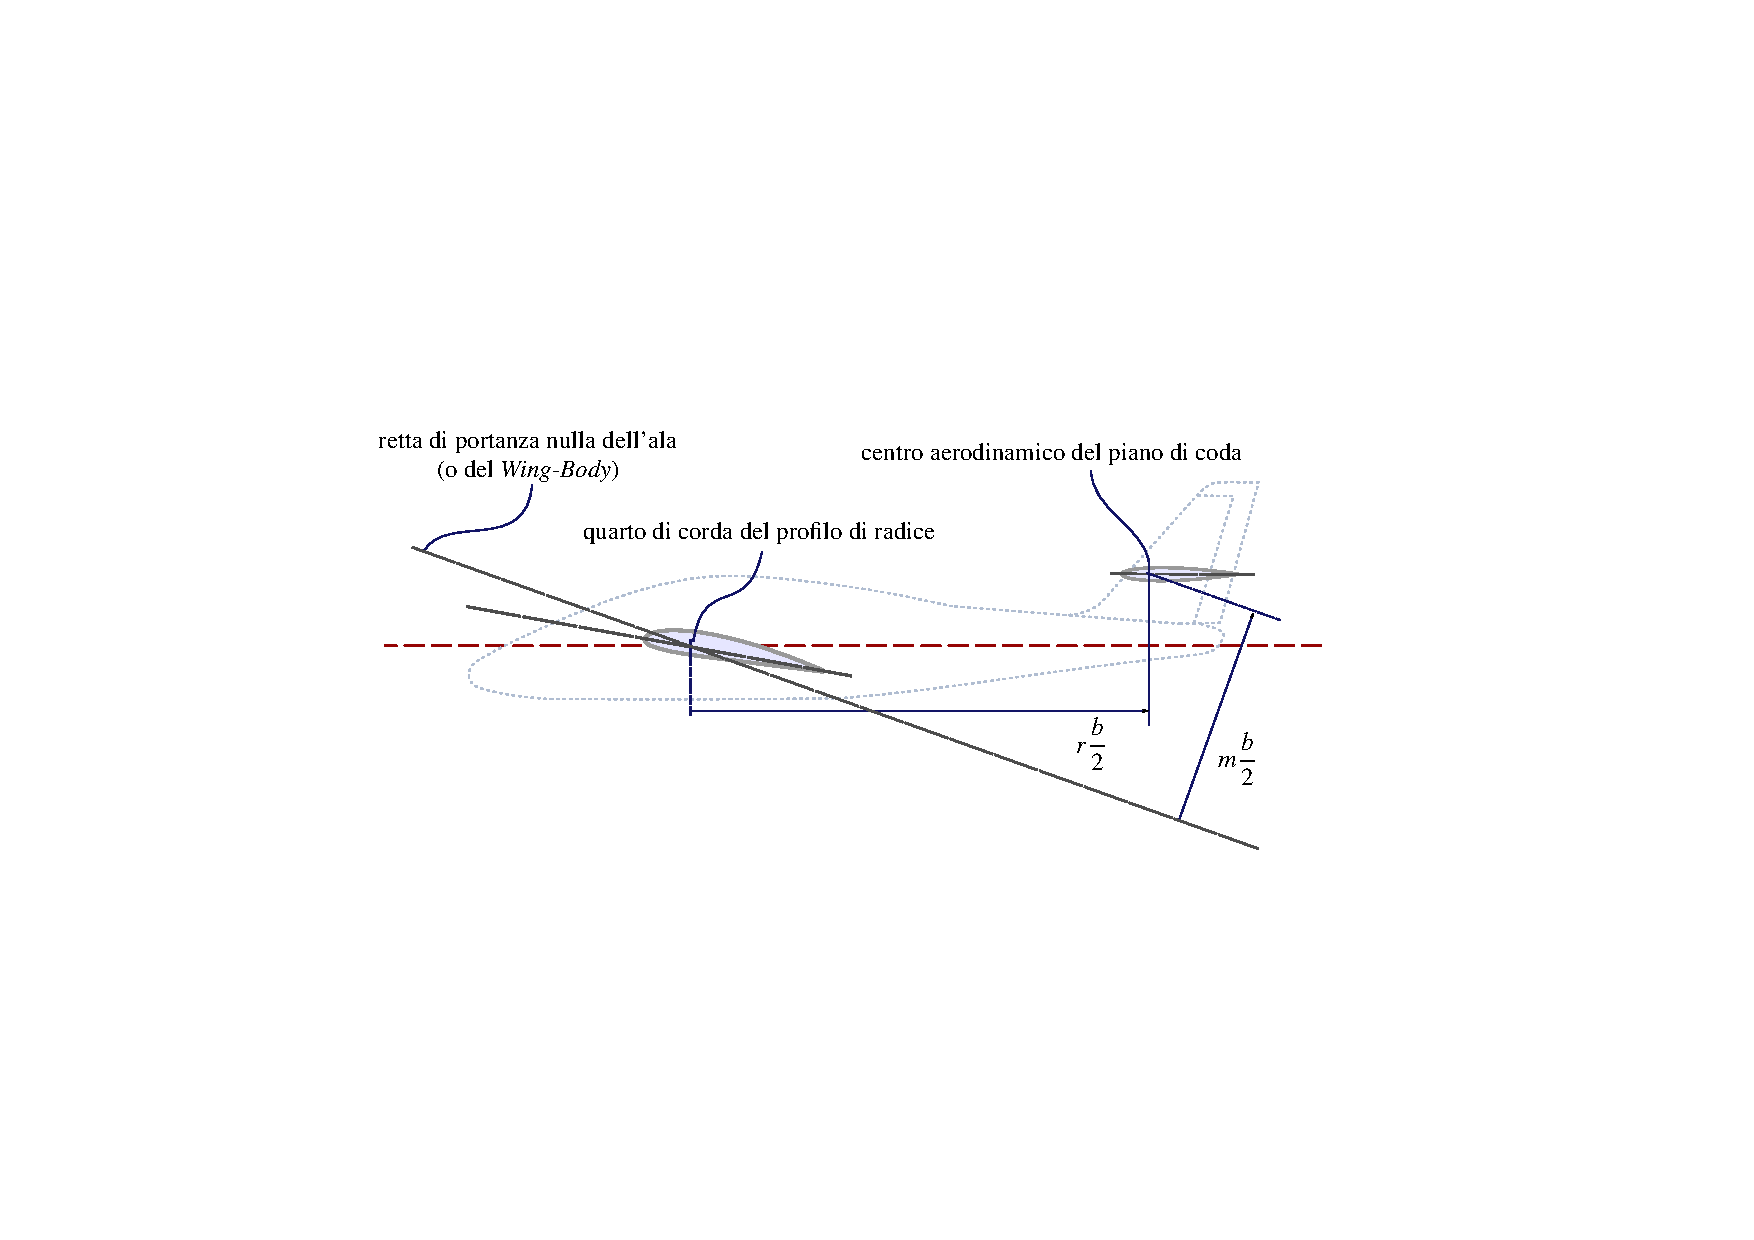
\includegraphics[height=7.3cm]{Immagini/wing_htail_Roskam.pdf}} 
\caption{Dimensions for determination of Downwash Gradient.}
\label{PerkinsDownwash}
\end{figure} 

%% METTI FONTE FORMULA DOWNWASH
%% TODO --> DIVIDI FORMULA \ALIGN


\begin{equation}
\begin{split}
 \frac{d\epsilon}{d\alpha} &= \frac{K_{\epsilon \Lambda}}{K_{\epsilon _{\Lambda=0}}}  \Biggr ( \frac{r}{r^2+m_{tv}^2} 
 \frac{0.4876}{\sqrt{r^2 + 0.6319 + m_{tv}^2}}  +\\
& \left [1+{ \left( \frac{r^2}{r^2 + 0.7915 + 5.0734 m_{tv}^2} \right) }^{0.3113}  \right ]    \left \{ 1- \sqrt{\frac{m_{tv}^2}{1+m_{tv}^2}} \right \}      \Biggl )    \frac{C_{L_{{\alpha}_w}}}{\pi \AR}
\end{split}
\end{equation}


Where the two $K_{\epsilon}$ terms accounting fot the wing sweep angle effect are defined as follow ( where $\Lambda $ expressed in radians):

\begin{equation}
K_{\epsilon \Lambda} = \frac{ 0.1124 + 0.1265 \Lambda + 0.1766 \Lambda^2}{r^2} + \frac{0.1024}{r} +2
\end{equation}

\begin{equation}
K_{\epsilon _{\Lambda=0}} = \frac{ 0.1124 }{r^2} + \frac{0.1024}{r} +2
\end{equation}

\section{Java Class Architecture}

In order to simplify the calculation of downwash, as mentioned, it's possible to assume the downwash gradient constant with the angle of attack. In this case the reference line to calculate the distance along z axis is the plane from the wing root chord or else the zero-lift line of the wing.\\
To obtain a more accurate analysis it's possible to consider the variation in alpha of the downwash gradient. So the reference line of wing it's not costant, but is the vortex sheed plane. The location of this plane depend from the value of downwash, but this location is itself necessary to evaluate the downwash. So it's necessary an iterative process in which the position of the vortex reference line at alpha is calculated from the value of downwash gradient at previous step.\\ 

In this process the reference angle of attack is the absolute angle $\alpha_a$, that is the angle between the flow direction and the zero lift line of the wing. This choice is necessary because for $\alpha_a = 0$ it's possible to assume the downwash zero, but the downwash gradient is not null.
In view of stability, however, the reference angle of attack is the $\alpha_B$. The relation between these angles is in the %fig. \ref{angle}. 

%FIGURA ANGOLI D ATTACCO

The downwash angle is calculated by a class named \texttt{DownwashCalculator}. The builder of this class defines and assings all the geometrical variables, necessary to implement the calculation. The  \texttt{DownwashCalculator} class has seven methods and some overloads. The methods are explained in the table~\ref{table:Table1}. The methods will be explained more in detail below.

\begin{table}[H]
\begin{tabular}{p{7cm}p{7.5cm}}
\toprule
 \\[0.1	cm] 
\lstinline[language=Java]!calculateDownwashGradientConstantDelft! & This method calculates the downwash gradient  considering the vertical distance geometrical and constant\\ \hline \\[0.1	cm] 
\lstinline[language=Java]!calculateDownwashNonLinearDelft! &This method calculates the downwash considering a non constant downwash gradient.  \\ \hline \\ [0.1cm]
\lstinline[language=Java]!getDownwashAtAlphaBody! & This method returns the value of downwash angle, interpolating data filled before.\\ \hline \\[0.1cm]
\lstinline[language=Java]!calculateZDistanceZeroLift!	& This method calculates the distance between the aerodynamic centre of horizontal tail and the zero lift line of the wing. \\ \hline \\[0.1cm]
\lstinline[language=Java]!Plot Methods ...! & Using these methods it's possible to plot the downwash angle, the downwash gradient and the distance in function of $\alpha_{B}$ \\
\bottomrule
\end{tabular}
\caption{Methods of \texttt{DownwashCalculator} class.}
\label{table:Table1}
\end{table}

% spiegazione delle classi nel dettaglio. Partire dal file user guide poi disegni.



%Starting from alpha absolute = 0. When alpha absolute =0, in fact, the value of downwash is assumed zero, but the downwash gradient
%is not null. The second step is for alphaabs = delta alpha. In order to evaluate the position of the vortex shed plane
%is used the value of downwash gradient at previous step as effort value. Starting from this position is calculated
%a new value of downwash gradient and a new value of downwash.
%schema
%foto

\subsection{Test Class}

\section{Developer's Guide}

% DEVELOPER GUIDE

